\subsubsection{Activation Functions}

From our observations, activation functions determines the shape of the fully connected neural network. With the one-dimensional data, the input and output of a neural network is always a scalar, which reveals interesting relations between the activation function and the output of neural network. We use two different activations functions to describe this relation.

\begin{figure}[!htb]
\begin{subfigure}[b]{0.5\textwidth}
	\centering
	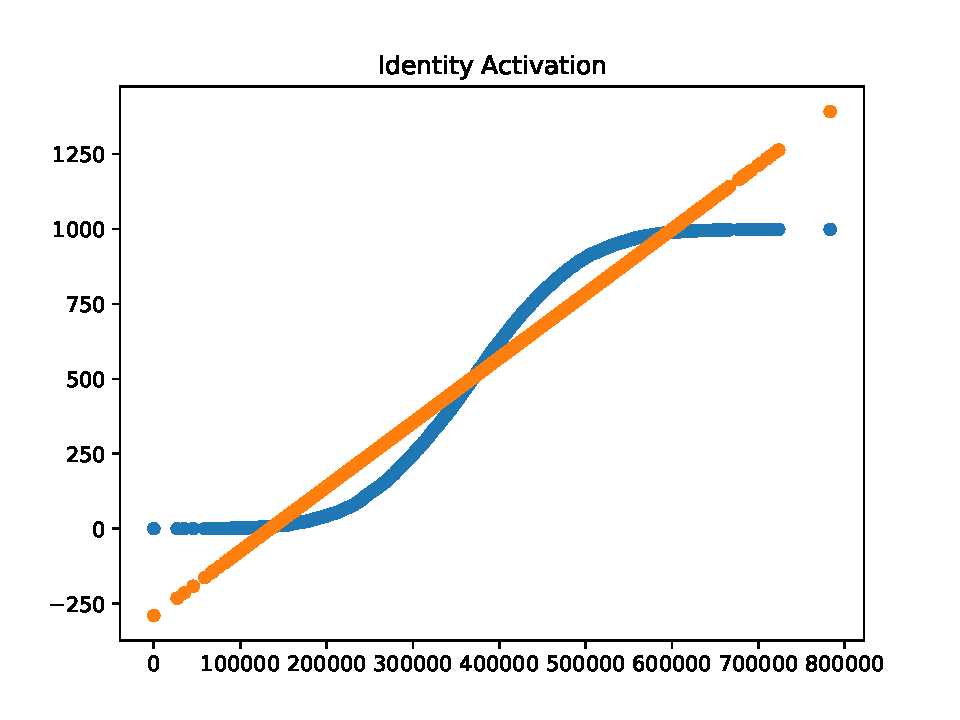
\includegraphics[width=8cm]{graphs/insights/identity}
	\caption{Identity Activation}
	\label{fig:id_act}
\end{subfigure}
\hfill
\begin{subfigure}[b]{0.5\textwidth}
	\centering
	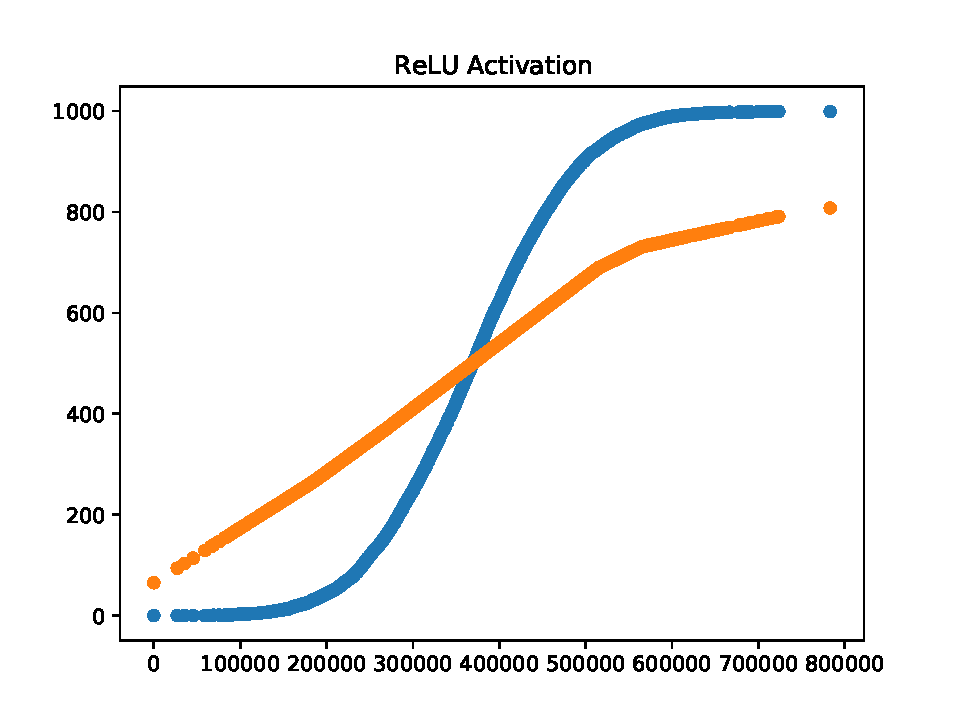
\includegraphics[width=8cm]{graphs/insights/relu}	
	\caption{ReLU Activation}
	\label{fig:relu_act}
\end{subfigure}
\caption{The predictions of neural networks with different activation functions. The blue line represents the ground truth and the orange line represents the predicted output.}
\label{fig:relation_of_activation_function}
\end{figure}

\begin{itemize}
\item
  If we use identity activation function, i.e.$z^{(i)}(x)=x$, then no
  matter how many layers are there, the fully connected neural network
  falls back to a linear regression.

  \textbf{Proof:} The output of the first layer, with identity activation function, will be $o^{(1)}=z^{(1)}(w^{(1)}x+b^{(1)})=w^{(1)}x+b^{(1)}$. Then the output will be the input of the next layer, and hence the output of the second layer will be $o^{(2)}=z^{(2)}(w^{(2)}(w^{(1)}x+b^{(1)})+b^{(2)})=w^{(2)}w^{(1)}x+w^{(2)}b^{(1)}+b^{(2)}$. Hence if we use identity activation, the trained neural network will become a linear regression. The predicted output of a neural network with identity activation is illustrated in Fig \ref{fig:id_act}, where we could verify that the predicted output is a line.
\item
  With ReLU (Rectified Linear Unit) as activation function, i.e. $z^{(i)}(x)=\text{max}(0,x)$, then the fully connected neural network becomes a piecewise linear function.

\textbf{Proof:} In the first layer, the output of a neural network with ReLU activation will be $o^{(1)}=z^{(1)}(w^{(1)}x+b^{(1)})=\text{max}(w^{(1)}x+b^{(1)},0)$. There will be two cases for this function:

\begin{equation}
	o^{(1)}=\begin{cases}	
		w^{(1)}x+b^{(1)} & w^{(1)}x+b^{(1)}>0 \\
		0 & \text{otherwise}
	\end{cases}
\end{equation}

\textbf{This paragraph will be rephrased very soon}

The output of the first layer will be the input of the second layer, which uses the same ReLU activation function. Hence the output will be $o^{(2)}=z^{(2)}(w^{(2)}o^{(1)}+b^{(2)})=z^{(2)}(w^{(2)}\text{max}(w^{(1)}x+b^{(1)},0)+b^{(2)})$. If $w^{(2)}(\text{max}(w^{(1)}x+b^{(1)},0))+b^{(2)}<0$, then the output will be $0$. Otherwise, as the $o^{(1)}$ is a vector, we have to perform the multiplication element by element. Assume that $o^{(1)}=[\text{max}(w^{(1)}_{1}x+b^{(1)}_1, 0),\cdots,\text{max}(w^{(1)}_{n}x+b^{(1)}_n,0)]$. By multiplying with $w^{(2)}$, we get $$o^{(2)}=w^{(2)}_1\text{max}(w_1^{(1)}x+b^{(1)}_1, 0)+\cdots+w^{(2)}_n\text{max}(w_n^{(1)}x+b^{(1)}_n, 0)+b_2$$

For each term in the equation above, there are two possibilities: $0$ when $w_i^{(1)}x+b_1<0$ or $w_i^{(2)}w_i^{(1)}x+w_i^{(2)}b_i^{(1)}$. Without loss of generality, we consider a case where all of them are non-zero. In this case, we will have $$o^{(2)}=\sum_{i}w_i^{(2)}w_i^{(1)}x+\sum_i w_i^{(2)}b_i^{(1)}+b_2$$ 

From the above induction, we find out that it is still a linear function when all values are positive. If there are some values to be zeros, then the function is still a linear function, but with different slope and intercept. Hence we conclude that the neural networks with ReLU activation function will become a piecewise linear function.

\end{itemize}